\section{Introduction}

Diffusion base models are generative models that had been invented 2015, same as GANs, but only gained popularity in 2020. Why that?

To refresh our mind, the goal of a generative model is to transform a simple distribution, like guassian, to a more complex one, that is close to the real world distribution, by means of a generator. The loss function measures the similarity between the two.

With VAEs, we compress the input data into a probabilistic latent space, from which we then sample. The stochastic nature of the sampling gives us the possibility to generate new sample. To do this,  we pick  a gaussian noise $\epsilon$ and we compute the random variable $z$ by multiplying its covariance and adding the mean  (\textbf{re-parametrization trick}).


Diffusion models differ a bit on what we have seen so far. The training can be divided into two parts:

\begin{enumerate}[H]
    \item \textbf{Forward Diffusion Process}: the content of an input image is "destroyed" by  adding noise over time $t$ to the image until data distribution becomes a Gaussian.

    \item \textbf{Reverse Diffusion Process}:  remove noise from the image.
\end{enumerate}

\subsection{Forward pass}

In order to approximate a Gaussian distribution, the added noise is incremented slightly at each step ($t$). To achieve a better approximation, the forward procedure requires \textbf{many iterations} ($t$). However, a trade-off arises: more steps lead to a better approximation but also increase the computational time required. Thus, selecting the number of steps is crucial, as it affects both the quality of the approximation and the computational resources needed.




\begin{figure}[!htbp]
    \centering
    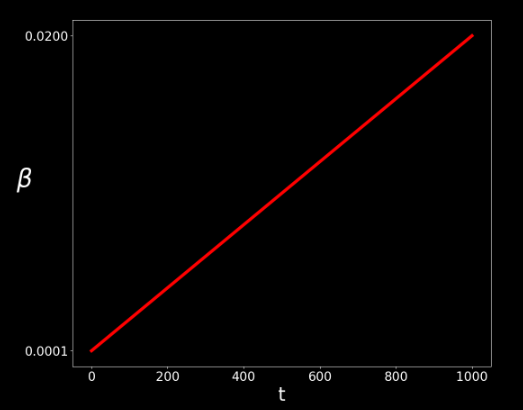
\includegraphics[width=\linewidth]{tikz/Diffusion models noise variance.png}
    \caption{{\color{red}\colorbox{pink}{Tikz TO-DO}} The figure shows the increment of the variance of noise, $\beta$, at each iteration. As we can seen, the increment is very little.}
    \label{fig:noise-variance}
\end{figure}

    
From figure   \ref{fig:diffusion-model} we can see that the forward procedure requires many intermidiate steps, each meaning the transition to one distribution to the other.



\begin{figure}[!htbp]
    \centering
    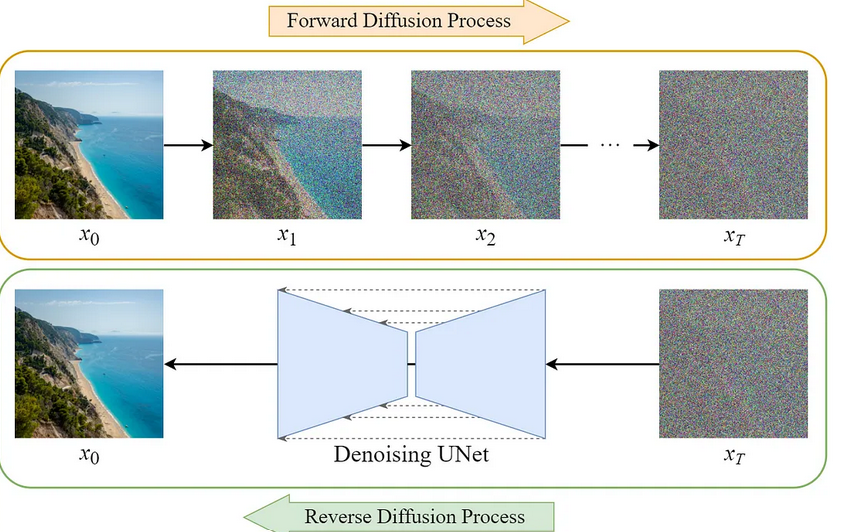
\includegraphics[width=\linewidth]{tikz/Diffusion Model.png}
    \caption{{\color{red}\colorbox{pink}{Tikz TO-DO}} Forward and Reverse pass in Diffusion Models}
    \label{fig:diffusion-model}
\end{figure}


The forward diffusion process gradually adds Gaussian noise to the input image $x_0$ step by step, and there will be $T$ steps in total. The process will produce a sequence of noisy image samples $x_1, \dots, x_T$. All the intermediate steps are gaussian distributed: $$q(x_{t}|x_{t-1}) = N(\sqrt{1-\beta_t}x_{t-1}, \beta_t I)$$

$\beta_t$ represents the increment of the variance of the noise at each timestep $t$.
The formula shows that, at each time, the new obtained gaussian is centered on the previous sample and rescaled by the variance of the added noise $\beta_t$. This allows to move toward a zero mean. If $\beta$ increase, then less data are maintained when the final gaussian is obtained  ($\sqrt{1-\beta_t}$), and more and more noise ($\beta_t I$)

When $T \longrightarrow \infty$, the final result will become a completely noisy image as if it is sampled from an \textbf{isotropic Gaussian distribution} ($\sum = \beta I$).

By defining $\alpha_t = (1- \beta_t)$, we can rewrite the formula as:

$$q(x_{t}|x_{t-1}) = N(\sqrt{\alpha_t}x_{t-1}, (1-\alpha_t) I)$$

When sampling all the steps sequentially, we need to compute the product of all the intermediate random variables:

$$q(x_{1:T}|x_0) = \prod_{t=1}^{T}q(x_t|x_{t-1})$$

Instead of designing an algorithm to compute this iteratively, we can use a closed-form formula for a Gaussian process to directly sample a noisy image (an intermediate step) at a specific time step $t$ by using the \textbf{reparameterization trick}\footnote{as seen in VAE, this step just requires to scale the variance by a constant and shift it by the shif parameter.} :


\begin{equation}
\begin{aligned}
    &\text{if } q(x_t|x_{t-1}) \sim N(\sqrt{\alpha_t}x_{t-1}, (1-\alpha_t) I) \\
    & 
    
    &x_t = \sqrt{\alpha_t}x_{t-1} + \sqrt{(1-\alpha_t)} \epsilon_{t-1}\text{ where } \epsilon \sim N(0,1)
\end{aligned}
\end{equation}

Then we can expand it recursively, unitll we get $x_0$, in order to obtain the closed-form formula:

\begin{figure}[!htbp]
    \centering
    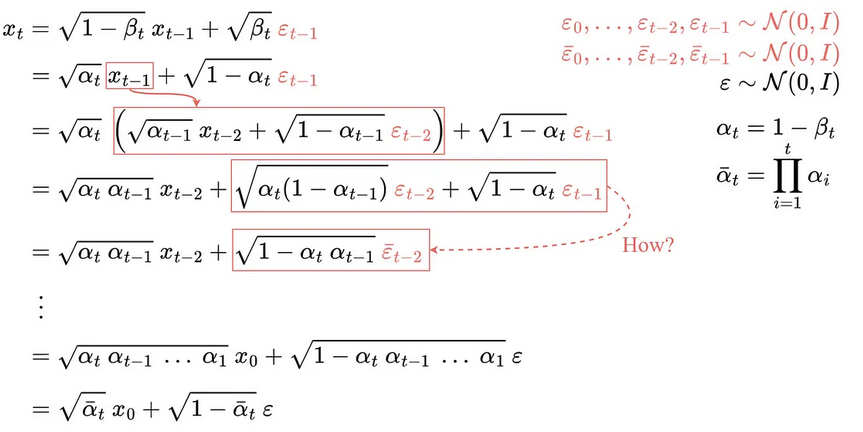
\includegraphics[width=1\linewidth]{tikz/diffusion model derivation.png}
    \caption{{\color{red}\colorbox{pink}{Tikz TO-DO}} The image shows the derivation of $x_t$ by recursively substitute $x_{t-1}$ untill $x_0$}
    \label{fig:enter-label}
\end{figure}

Thus:

$$x_t \sim N(\sqrt{\overline{\alpha}}_t x_0, (1- \overline{\alpha}_t)I) \text{   where } \overline{\alpha}_t = \prod_{t=1}^{T}\alpha_t$$

And by applying the re-parametrization trick we get its close formula:

$$x_t = \sqrt{\overline{\alpha}_t}x_{0} + \sqrt{1- \overline{\alpha}_t}\epsilon_0$$



As we can see, the final formula depends only on the input image $x_0$. This has a significant implication: it allows us to directly sample $x_t$ at \textbf{any time step}, making the forward process much faster since we do not have to compute the entire product of all timesteps. The meaning is that we can sample any intermediate sample $x_t$ by simply multiply all the $\alpha_{t}$ along the way ($\overline{\alpha}_t = \prod_{t=1}^{T}\alpha_t$). As t approaches T, at the end we get an (almost surely) Gaussian Distribution.


\subsection{Reverse pass}

So far, we have seen how to destroy all the image data using efficient transformations, but this procedure does not involve any training. What we are missing is an understanding of how the model can generate a sample from this final Gaussian distribution. Specifically, how does the model learn to reverse the process and transform noise back into the original data distribution?

\begin{figure}[H]
    \centering
    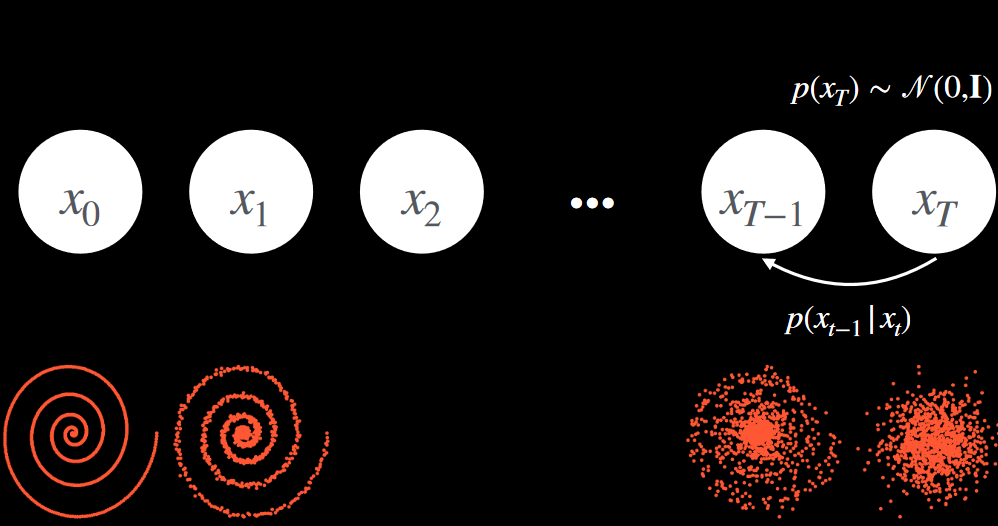
\includegraphics[width=0.75\linewidth]{tikz/Reverse process.png}
    \caption{An example of the reverse process}
    \label{fig:reverse-process}
\end{figure}

Unlike the forward process, we cannot use $p(x_{t-1}|x_t)$ to reverse the noise since the denominator ($p(x_t)$) and the marginal distribution of an intermediate step ($p(x_{t-1}$)) are intractable:

$$p(x_{t-1}|x_t)=\frac{p(x_t|x_{t-1})p(x_{t-1})}{p(x_t)}$$

Thus we need to train a neural network $p_{\theta}(x_{t-1}|x_{t})$ to approximate the reverse process $p(x_{t-1}|x_t)$ (i.e. to approximate the posterior distribution ... sounds familiar?). The approximation $p_{\theta}(x_{t-1}|x_{t})$ follows a normal distribution (\textbf{the reverse of a gaussian process is still a gaussian distribution}) and the network learns \textbf{only} the $\mu_{\theta}$ of the reverse gaussian process, as the the variance is fixed, i.e. is shared among the intermediate reverse steps \footnote{OpenAI saw that learning the variance does not provide improvements, thanks God.}: 

$$P_{\theta}(x_{t-1}|x_t) = N(\mu_{\theta}(x_t,t), \sum_{t})$$

As you may have already understood, diffusion models can be seen as a special case of hierarchical VAEs, but:
\begin{itemize}
    \item The encoder is fixed (it’s the forward process)
    \item Latent variables have the same dimensionality of data

    \item The same model is applied across different
timesteps
\end{itemize}

With this set up, instead of optimizing the intractable loss function itself, we can optimize the Variational Lower Bound. At the end, similar to VAEs, the Neural Network can be trained with \textbf{ELBO}:

\begin{equation}
\mathcal{L} = \mathbb{E}_{q(x_1 | x_0)} \left[ \log p_{\theta}(x_0 | x_1) \right] - \sum_{t=2}^{T} \mathbb{E}_{q(x_t | x_0)} \left[ D_{KL} \left[ q(x_{t-1} | x_t, x_0) \| p_{\theta}(x_{t-1} | x_t) \right] \right]
\end{equation}

The loss compares intermediate steps with a boundary condition (first term) and computes the KL divergence between the distributions of every reverse step. As the distribution of each reverse step is assumed to be a gaussian, we can use the close formula of KL:



%\begin{figure}[!htbp]
%    \centering
%    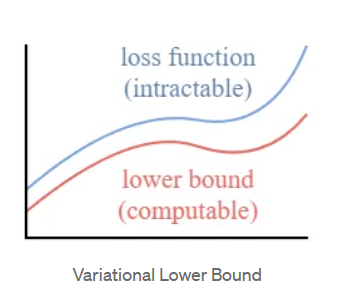
\includegraphics[width=\linewidth]{tikz/lower bound.png}
%    \caption{{\color{red}\colorbox{pink}{Tikz TO-DO}} Lower bound for log likelihood}
%    \label{fig:enter-label}
%\end{figure}

$$\frac{1}{2\sigma^2_q(t)}||\mu_{\theta}-\mu_q||^2_2$$

This is the original formulation from 2015. To better explain it, recall that the reverse process, which the model learns, involves denoising the data step-by-step to reconstruct the original data distribution. Thus, this terms aims at training a diffusion model to \textbf{remove noise from data}. It does so by minimizing the discrepancy between the predicted and true means at each step, scaled by a variance term. The goal of this loss term is to measure how close the predicted mean $\mu_\theta$ is to the true mean $\mu_q$ \footnote{ This is the true mean of the data at a given time step $t$, according to the forward diffusion process.} at each step of the diffusion process. By minimizing this term during training, the model learns to better approximate the true mean of the data distribution as it progresses through the diffusion steps. 

However, the formula was updated in 2020 to enhance the efficiency and effectiveness of the noise removal process:

$$||\epsilon - \hat{\epsilon}_{\theta}(x_t,t)||^{2}_2$$

The updated formula simplifies the process by focusing directly on the difference in the added noise. Here,  $\epsilon$ \footnote{In the context of diffusion models, $\epsilon$ represents the actual noise that was added to the original data to obtain the noisy data at time step $t$.} represents the true total added noise up to timestep $t$, while $\hat{\epsilon}_{\theta}$ is the noise predicted by the model parameterized by $\theta$. The function $\hat{\epsilon}_{\theta}$ takes the noisy data $x_t$ and the time step $t$ as inputs and outputs an estimate of the noise that was added to the data. Then, the model measures and try to minimize the squared difference between the true noise  and the model's predicted noise. The goal is to learn to accurately estimate the noise that was added to the data at each time step $t$, making the process a \textbf{true noise removal process}.

Talking about the \textbf{Boundary condition} (first term), it can be also described through the added noise:

$$\log p_{\theta}(x_0|x_1) = - || \epsilon_{0}-\epsilon_{\theta}(x_1, 1)||^{2}_2$$

This is the log probability of the original data $x_0$ given the noisy data $x_1$, according to the model parameterized by $\theta$. It represents how well the model can reconstruct $x_0$ from $x_1$, by using the L2 norm between the true and predicted noise, respectivelly $\epsilon_{0}$ and $\epsilon_{\theta}(x_1, 1)$. By using this term, the model learns how to predict the amount of noise added to the initial data ($x_0$).


To define the lower bound of the log-likelihood of a sample, we can re-write the loss as follows\footnote{just substitute to $D_{KL}$ and $log p_{theta}(x_0|x_1)$ the previous transformations}:

$$\log p(x_0) \geq - \sum_{t=1}^{T} E_{q(x_t|x_0)}||\epsilon - \epsilon_{\theta}(x_t,t)||^2_2$$ 

Furthermore, compute all timesteps for each sample is computationally expensive (as we have to predict the noisy for each reverse process for each sample), so we use a Monte Carlo approximation:

$$L = E_{x_0 \sim q(x_0), \epsilon \sim N(0,1), t \sim U(1,T)} ||\epsilon - \epsilon_{\theta}(\sqrt{\hat{\alpha_t}}x_0 + \sqrt{(1-\hat{\alpha_t})}\epsilon, t)||^{2}_2$$

In practice, we select a random sample $x_0$, add noise $\epsilon$, choose a random timestep $t$ along the trajectory, and calculate the added noise, comparing it with the actual $\epsilon$.


The reverse process, which removes the added noise, is described by the following close formula (use the parametrization trick):

$$x_{t-1}= \frac{1}{\sqrt{\alpha_t}}(x_t - \frac{\beta_t}{\sqrt{1-\hat{\alpha_t}}}\epsilon_{\theta}(x_t,t))+\sigma_t z$$

We have finally obtained an efficient formula that achieves the training goal: \textbf{an iterative process that enables the model to transform noisy data into clean data by progressively removing the estimated noise}.

\subsection{Generative Trilemma}

In the context of generative models, there exists a trilemma based on three properties: \textit{fast sampling}, \textit{diversity}, and \textit{high-quality samples}. Different types of generative models (VAEs, GANs, and diffusion models) excel in different combinations of these properties:

\begin{itemize}
    \item \textbf{VAEs}: Fast sampling and diversity.
    \item \textbf{GANs}: Fast sampling and high quality.
    \item \textbf{Diffusion Models}: High quality and diversity.
\end{itemize}

Recently, diffusion models have also made significant advancements in fast sampling, attempting to balance all three properties.

\begin{figure}[H]
    \centering
    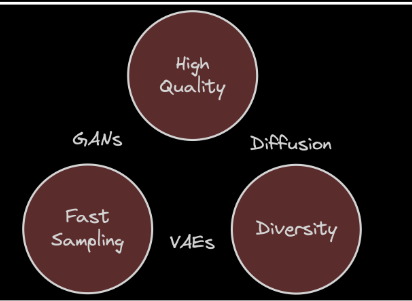
\includegraphics[width=0.75\linewidth]{tikz/Generative trilemma.png}
    \caption{generative trilemma}
    \label{fig:generative-trilemma}
\end{figure}

\subsection{Forward Process and stocastich equation}

The forward process is defined as:

$$x_t = \sqrt{(1- \beta_t)}x_{t-1} + \sqrt{\beta_t}\epsilon \text{ with } \epsilon \sim N(0,I)$$

As we take smaller and smaller steps, $\beta$ can be rewritten as a continuous function:

$$x_t = \sqrt{(1- \beta(t)\Delta t})x_{t-1} + \sqrt{\beta(t)\Delta t}\epsilon \text{ with } \epsilon \sim N(0,I)$$

Using Taylor expansion, we get a stochastic differential equation:

$$dx_t = - \frac{1}{2}\beta(t)x_t dt + \sqrt{\beta(t)}dw_t$$

The first part is the drift term, and the second is the diffusion term. The reverse process is given by:

$$dx_t = \left[-\frac{1}{2}\beta(t)x_t -\beta(t)\nabla_{x_{t}} \log q_t(x_t) \right]dt + \sqrt{\beta(t)}d\hat{w}_t$$

The logarithmic term, called the score, indicates where the data is more concentrated.

\subsection{Denoising Score Matching}

Training the diffusion model can be formulated as:

$$\min_{\theta} = E_{x_0 \sim q(x_0), \epsilon \sim N(0,I), t \sim U(1,T)} \left[ \frac{\lambda(t)}{\sigma^2_t}||\epsilon - \epsilon_{\theta}(x_t,t)||^2\right]$$

This formulation allows interpolating latent spaces, resulting in continuous and semantically meaningful changes in the data space.

\subsection{Network Architecture}

The network used is similar to the pix2pix model, with Fourier features used to encode the timestep information. These features are typically sinusoidal functions (sine and cosine) that help represent the temporal information in a more expressive way (like in positional embedding). Additionally, Vision transformers (ViTs) can be employed to leverage self-attention mechanisms, enhancing the model's ability to capture complex patterns and relationships in images.

\begin{figure}[!htbp]
    \centering
    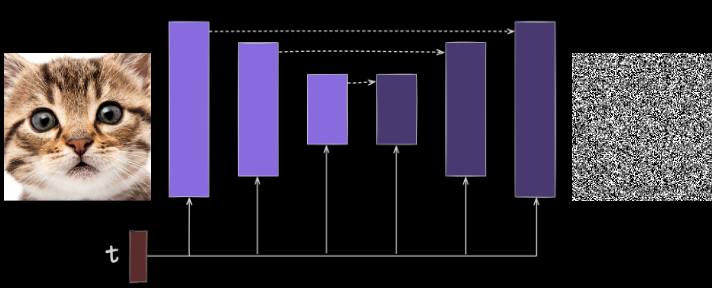
\includegraphics[width=\linewidth]{tikz/diffusion model architecture.png}
    \caption{{\color{red}\colorbox{pink}{Tikz TO-DO}} Diffusion model architecture}
    \label{fig:enter-label}
\end{figure}

\section{Text Conditioning}

To model the probability of a sample given conditioning, we decompose the chain as follows:

$$p(x|c)= p(x_T)\prod_{t=1}^{T}p_{\theta}(x_{t-1}|x_t,c)$$


So do we need to just train an extra conditional model $ p_{\theta}(x_{t-1}|x_t,c)$? Unfortunately, this approach does not work effectively because the network tends to ignore the conditional signals over the chain, leading to a behavior similar to unconditional learning. OpenAI addressed this issue by introducing a bias on top of the predictions. This method involves considering the probability of the condition given the sample, the probability of the sample, and the probability of the condition.

$$p(x|c)= \frac{p(c|x)p(x)}{p(c)}$$

We can log it:

$$logp(x|c)= log \frac{p(c|x)p(x)}{p(c)}$$
$$logp(x|c)= log p(c|x) + log p(x) -log p(c)$$

If we take the derivative in respect of our sample x, we would see that the probability of the bias term $p(c)$ does not depends on x:

$$\nabla_x p(x|c)= \nabla_x  p(c|x) + \nabla_x  p(x) - \nabla_x  p(c)$$

Thus, we can rule out the third term. At the end, the probability of our sample given the condition becames the probability of the sample itselfe ($p(x)$, unconditional score of previous diffusion model) plus classifier score ($p(c|x)$):

$$\nabla_x p(x|c)= \nabla_x  p(c|x) + \nabla_x  p(x)$$

We can sharpen the conditioning at the expense of diversity :

$$\nabla_x  p(x|c)= \gamma \nabla_x  p(c|x) + \nabla_x p(x) $$

This setting requires a trained external noisy classifier for computing the classifier score $p(c|x)$. Do we really need it? Nope, because we could take the classifier score and reapplied bias on top of it \footnote{reapply the bayesian theorem and log it.}:

$$ \nabla_x  p(c|x)  = \nabla_x  p(x|c) + \nabla_x p(c) - \nabla_x p(x)$$

Once again, $ \nabla_x p(c)$ does not depend of x, thus it can be ruled out. 

$$ \nabla_x  p(c|x)  = \nabla_x  p(x|c) - \nabla_x  p(x)$$

If we plug back, then:

$$\nabla_x  p(x|c)= \gamma(\nabla_x  p(x|c) - \nabla_x  p(x))+ \nabla_x  p(x) $$
$$\nabla_x  p(x|c)= \gamma\nabla_x  p(x|c) + (1-\gamma)\nabla_x  p(x) $$

We have a linear combination of the gradients of the conditional and unconditional models, respectivelly $\nabla_x  p(x|c)$ and $\nabla_x  p(x)$. This combination allows the model to incorporate both the conditional information and the general behavior of x. By adjusting $\gamma$, one can control the influence of the conditional information versus the unconditional information. We are back in using just one network trained in two fashions, one conditioned and one unconditioned. Thus, no external classifier is needed

How do we inject text?

\subsection{Stable diffusion}

Stable Diffusion refers to a technique in generative models that involves encoding and decoding image data to manage the computational complexity of the diffusion process. Directly computing the diffusion process in the pixel space, which is the high-dimensional space of the original image, is computationally expensive. To address this challenge, the image data is first compressed into a lower-dimensional latent space. This compression is achieved using an encoder, which transforms the high-dimensional pixel data into a more manageable latent representation.

Once the image data is in this lower-dimensional latent space, the diffusion process—where noise is added and removed to gradually generate an image—is performed. This makes the process significantly more computationally efficient. After the diffusion process is completed in the latent space, a decoder is used to reconstruct the image data back into the original pixel space. This ensures that the final output is a high-quality image that accurately represents the original data.

The architecture used in the reverse process is typically an autoencoder, specifically \textbf{U-Net}: The U-Net consists of an encoder  and a decoder with skip connections between corresponding layers in the encoder and decoder. U-Nets are capable of effectively removing noise while preserving important details in the image, as Skip connections help retain high-resolution details.

This process is also called \textbf{Denoising U-Net}:

\begin{itemize}
    \item \textbf{Encoder}: Captures features and reduces spatial dimensions.
    \item \textbf{Bottleneck}: Holds the most abstract features.
    \item \textbf{Decoder}: Reconstructs the image at each timestep, increasing spatial dimensions.
\end{itemize}


Additionally, stable diffusion models often incorporate a conditioning space. This space includes additional information that guides the diffusion process. For instance, in conditional generative models, this conditioning information could be labels, textual descriptions, or other contextual data that influence the generation of the images. By integrating this conditioning information, the diffusion process can produce outputs that are aligned with the given conditions. This integration can be achieved by concatenating the conditioning information with the latent representation or through other mechanisms within the network.



\begin{figure}[H]
    \centering
    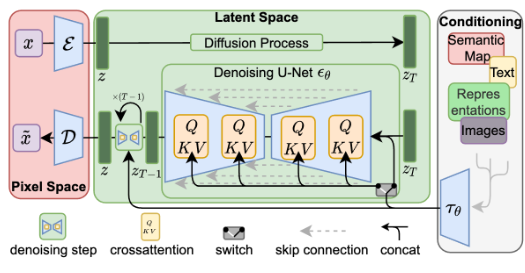
\includegraphics[width=\linewidth]{tikz/A.png}
    \caption{{\color{red}\colorbox{pink}{Tikz TO-DO}} Enter Caption}
    \label{fig:enter-label}
\end{figure}


\begin{figure}{H}
    \centering
    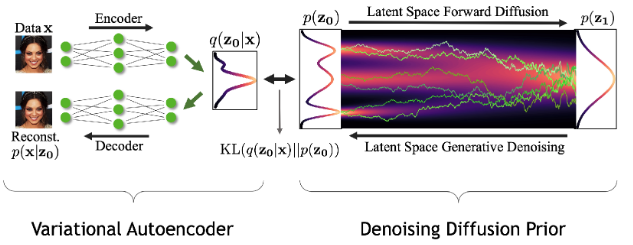
\includegraphics[width=\linewidth]{tikz/B.png}
    \caption{{\color{red}\colorbox{pink}{Tikz TO-DO}} Enter Caption}
    \label{fig:enter-label}
\end{figure}


